\section{Introduction}



\begin{frame}{Introduction}
 \begin{columns}

% Left column
\begin{column}{0.5\textwidth}
\begin{tcolorbox}[
    colback=white,
    colframe=blue,
    colbacktitle=blue!50!black!50,
    title=Astrophysical Relevance of BNS, 
    fonttitle=\bfseries,
    rounded corners,
    boxrule=1pt,
    left=2mm, right=2mm, top=1mm, bottom=1mm
]
    \begin{itemize}
    \scriptsize
    \item Gravitational Waves
    \item Electromagnetic Radiation
    \item Neutrino Emission
    \item Nucleosynthesis
    %\begin{itemize}
     %   \scriptsize
      %  \item $r$-process site
      %  \item Formation radioactive isotopes
       % \item Decay powering Kilonovae 
    %\end{itemize}
\end{itemize}

\end{tcolorbox}
\end{column}

% Right column
\begin{column}{0.5\textwidth}

\begin{tcolorbox}[
    colback=white,
    colframe=blue,
    colbacktitle=blue!50!black!50,
    title=Motivations and Goals,
    fonttitle=\bfseries,
    rounded corners,
    boxrule=1pt,
    left=2mm, right=2mm, top=1mm, bottom=1mm
]
\begin{itemize}
   \scriptsize
    \item Multiple Scales guiding the problem
     %\begin{itemize}
     %	\scriptsize
	%\item Merger Dynamics: ms time-scale
	%\item Ejecta Expansion : year time-scale
	%\item Light Curve : days to months time-scale
	%\item Weak forces ms to sec time-scale
    %\end{itemize}
    %\scriptsize
    \item High costs of long NR simulations
    \item Large d.o.f. of nuclear networks
    \item Goal : bridge the gap between these different regimes
\end{itemize}
\end{tcolorbox}

\end{column}


\end{columns}
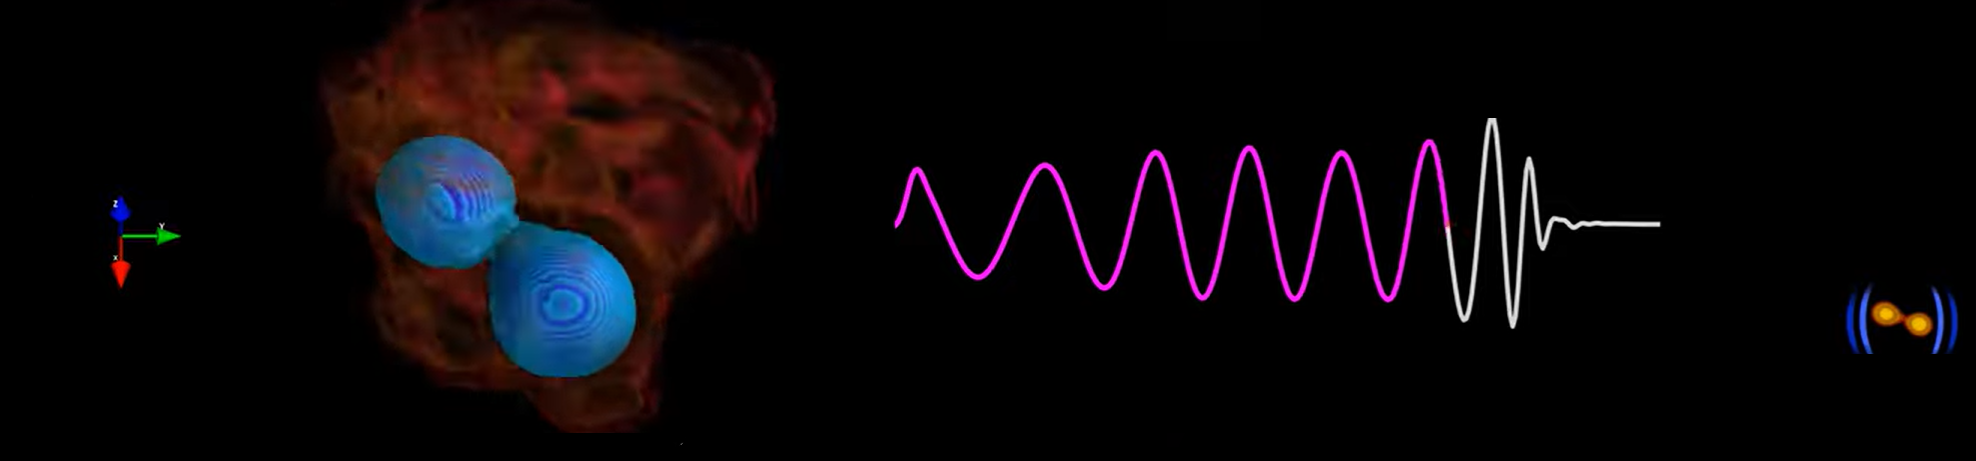
\includegraphics[width=\linewidth]{../fig/merger.png}

\end{frame}